
% Default to the notebook output style

    


% Inherit from the specified cell style.




    
\documentclass[11pt]{article}

    
    
    \usepackage[T1]{fontenc}
    % Nicer default font (+ math font) than Computer Modern for most use cases
    \usepackage{mathpazo}

    % Basic figure setup, for now with no caption control since it's done
    % automatically by Pandoc (which extracts ![](path) syntax from Markdown).
    \usepackage{graphicx}
    % We will generate all images so they have a width \maxwidth. This means
    % that they will get their normal width if they fit onto the page, but
    % are scaled down if they would overflow the margins.
    \makeatletter
    \def\maxwidth{\ifdim\Gin@nat@width>\linewidth\linewidth
    \else\Gin@nat@width\fi}
    \makeatother
    \let\Oldincludegraphics\includegraphics
    % Set max figure width to be 80% of text width, for now hardcoded.
    \renewcommand{\includegraphics}[1]{\Oldincludegraphics[width=.8\maxwidth]{#1}}
    % Ensure that by default, figures have no caption (until we provide a
    % proper Figure object with a Caption API and a way to capture that
    % in the conversion process - todo).
    \usepackage{caption}
    \DeclareCaptionLabelFormat{nolabel}{}
    \captionsetup{labelformat=nolabel}

    \usepackage{adjustbox} % Used to constrain images to a maximum size 
    \usepackage{xcolor} % Allow colors to be defined
    \usepackage{enumerate} % Needed for markdown enumerations to work
    \usepackage{geometry} % Used to adjust the document margins
    \usepackage{amsmath} % Equations
    \usepackage{amssymb} % Equations
    \usepackage{textcomp} % defines textquotesingle
    % Hack from http://tex.stackexchange.com/a/47451/13684:
    \AtBeginDocument{%
        \def\PYZsq{\textquotesingle}% Upright quotes in Pygmentized code
    }
    \usepackage{upquote} % Upright quotes for verbatim code
    \usepackage{eurosym} % defines \euro
    \usepackage[mathletters]{ucs} % Extended unicode (utf-8) support
    \usepackage[utf8x]{inputenc} % Allow utf-8 characters in the tex document
    \usepackage{fancyvrb} % verbatim replacement that allows latex
    \usepackage{grffile} % extends the file name processing of package graphics 
                         % to support a larger range 
    % The hyperref package gives us a pdf with properly built
    % internal navigation ('pdf bookmarks' for the table of contents,
    % internal cross-reference links, web links for URLs, etc.)
    \usepackage{hyperref}
    \usepackage{longtable} % longtable support required by pandoc >1.10
    \usepackage{booktabs}  % table support for pandoc > 1.12.2
    \usepackage[inline]{enumitem} % IRkernel/repr support (it uses the enumerate* environment)
    \usepackage[normalem]{ulem} % ulem is needed to support strikethroughs (\sout)
                                % normalem makes italics be italics, not underlines
    

    
    
    % Colors for the hyperref package
    \definecolor{urlcolor}{rgb}{0,.145,.698}
    \definecolor{linkcolor}{rgb}{.71,0.21,0.01}
    \definecolor{citecolor}{rgb}{.12,.54,.11}

    % ANSI colors
    \definecolor{ansi-black}{HTML}{3E424D}
    \definecolor{ansi-black-intense}{HTML}{282C36}
    \definecolor{ansi-red}{HTML}{E75C58}
    \definecolor{ansi-red-intense}{HTML}{B22B31}
    \definecolor{ansi-green}{HTML}{00A250}
    \definecolor{ansi-green-intense}{HTML}{007427}
    \definecolor{ansi-yellow}{HTML}{DDB62B}
    \definecolor{ansi-yellow-intense}{HTML}{B27D12}
    \definecolor{ansi-blue}{HTML}{208FFB}
    \definecolor{ansi-blue-intense}{HTML}{0065CA}
    \definecolor{ansi-magenta}{HTML}{D160C4}
    \definecolor{ansi-magenta-intense}{HTML}{A03196}
    \definecolor{ansi-cyan}{HTML}{60C6C8}
    \definecolor{ansi-cyan-intense}{HTML}{258F8F}
    \definecolor{ansi-white}{HTML}{C5C1B4}
    \definecolor{ansi-white-intense}{HTML}{A1A6B2}

    % commands and environments needed by pandoc snippets
    % extracted from the output of `pandoc -s`
    \providecommand{\tightlist}{%
      \setlength{\itemsep}{0pt}\setlength{\parskip}{0pt}}
    \DefineVerbatimEnvironment{Highlighting}{Verbatim}{commandchars=\\\{\}}
    % Add ',fontsize=\small' for more characters per line
    \newenvironment{Shaded}{}{}
    \newcommand{\KeywordTok}[1]{\textcolor[rgb]{0.00,0.44,0.13}{\textbf{{#1}}}}
    \newcommand{\DataTypeTok}[1]{\textcolor[rgb]{0.56,0.13,0.00}{{#1}}}
    \newcommand{\DecValTok}[1]{\textcolor[rgb]{0.25,0.63,0.44}{{#1}}}
    \newcommand{\BaseNTok}[1]{\textcolor[rgb]{0.25,0.63,0.44}{{#1}}}
    \newcommand{\FloatTok}[1]{\textcolor[rgb]{0.25,0.63,0.44}{{#1}}}
    \newcommand{\CharTok}[1]{\textcolor[rgb]{0.25,0.44,0.63}{{#1}}}
    \newcommand{\StringTok}[1]{\textcolor[rgb]{0.25,0.44,0.63}{{#1}}}
    \newcommand{\CommentTok}[1]{\textcolor[rgb]{0.38,0.63,0.69}{\textit{{#1}}}}
    \newcommand{\OtherTok}[1]{\textcolor[rgb]{0.00,0.44,0.13}{{#1}}}
    \newcommand{\AlertTok}[1]{\textcolor[rgb]{1.00,0.00,0.00}{\textbf{{#1}}}}
    \newcommand{\FunctionTok}[1]{\textcolor[rgb]{0.02,0.16,0.49}{{#1}}}
    \newcommand{\RegionMarkerTok}[1]{{#1}}
    \newcommand{\ErrorTok}[1]{\textcolor[rgb]{1.00,0.00,0.00}{\textbf{{#1}}}}
    \newcommand{\NormalTok}[1]{{#1}}
    
    % Additional commands for more recent versions of Pandoc
    \newcommand{\ConstantTok}[1]{\textcolor[rgb]{0.53,0.00,0.00}{{#1}}}
    \newcommand{\SpecialCharTok}[1]{\textcolor[rgb]{0.25,0.44,0.63}{{#1}}}
    \newcommand{\VerbatimStringTok}[1]{\textcolor[rgb]{0.25,0.44,0.63}{{#1}}}
    \newcommand{\SpecialStringTok}[1]{\textcolor[rgb]{0.73,0.40,0.53}{{#1}}}
    \newcommand{\ImportTok}[1]{{#1}}
    \newcommand{\DocumentationTok}[1]{\textcolor[rgb]{0.73,0.13,0.13}{\textit{{#1}}}}
    \newcommand{\AnnotationTok}[1]{\textcolor[rgb]{0.38,0.63,0.69}{\textbf{\textit{{#1}}}}}
    \newcommand{\CommentVarTok}[1]{\textcolor[rgb]{0.38,0.63,0.69}{\textbf{\textit{{#1}}}}}
    \newcommand{\VariableTok}[1]{\textcolor[rgb]{0.10,0.09,0.49}{{#1}}}
    \newcommand{\ControlFlowTok}[1]{\textcolor[rgb]{0.00,0.44,0.13}{\textbf{{#1}}}}
    \newcommand{\OperatorTok}[1]{\textcolor[rgb]{0.40,0.40,0.40}{{#1}}}
    \newcommand{\BuiltInTok}[1]{{#1}}
    \newcommand{\ExtensionTok}[1]{{#1}}
    \newcommand{\PreprocessorTok}[1]{\textcolor[rgb]{0.74,0.48,0.00}{{#1}}}
    \newcommand{\AttributeTok}[1]{\textcolor[rgb]{0.49,0.56,0.16}{{#1}}}
    \newcommand{\InformationTok}[1]{\textcolor[rgb]{0.38,0.63,0.69}{\textbf{\textit{{#1}}}}}
    \newcommand{\WarningTok}[1]{\textcolor[rgb]{0.38,0.63,0.69}{\textbf{\textit{{#1}}}}}
    
    
    % Define a nice break command that doesn't care if a line doesn't already
    % exist.
    \def\br{\hspace*{\fill} \\* }
    % Math Jax compatability definitions
    \def\gt{>}
    \def\lt{<}
    % Document parameters
    \title{CA\_Assignment3\_Jose\_modified}
    
    
    

    % Pygments definitions
    
\makeatletter
\def\PY@reset{\let\PY@it=\relax \let\PY@bf=\relax%
    \let\PY@ul=\relax \let\PY@tc=\relax%
    \let\PY@bc=\relax \let\PY@ff=\relax}
\def\PY@tok#1{\csname PY@tok@#1\endcsname}
\def\PY@toks#1+{\ifx\relax#1\empty\else%
    \PY@tok{#1}\expandafter\PY@toks\fi}
\def\PY@do#1{\PY@bc{\PY@tc{\PY@ul{%
    \PY@it{\PY@bf{\PY@ff{#1}}}}}}}
\def\PY#1#2{\PY@reset\PY@toks#1+\relax+\PY@do{#2}}

\expandafter\def\csname PY@tok@w\endcsname{\def\PY@tc##1{\textcolor[rgb]{0.73,0.73,0.73}{##1}}}
\expandafter\def\csname PY@tok@c\endcsname{\let\PY@it=\textit\def\PY@tc##1{\textcolor[rgb]{0.25,0.50,0.50}{##1}}}
\expandafter\def\csname PY@tok@cp\endcsname{\def\PY@tc##1{\textcolor[rgb]{0.74,0.48,0.00}{##1}}}
\expandafter\def\csname PY@tok@k\endcsname{\let\PY@bf=\textbf\def\PY@tc##1{\textcolor[rgb]{0.00,0.50,0.00}{##1}}}
\expandafter\def\csname PY@tok@kp\endcsname{\def\PY@tc##1{\textcolor[rgb]{0.00,0.50,0.00}{##1}}}
\expandafter\def\csname PY@tok@kt\endcsname{\def\PY@tc##1{\textcolor[rgb]{0.69,0.00,0.25}{##1}}}
\expandafter\def\csname PY@tok@o\endcsname{\def\PY@tc##1{\textcolor[rgb]{0.40,0.40,0.40}{##1}}}
\expandafter\def\csname PY@tok@ow\endcsname{\let\PY@bf=\textbf\def\PY@tc##1{\textcolor[rgb]{0.67,0.13,1.00}{##1}}}
\expandafter\def\csname PY@tok@nb\endcsname{\def\PY@tc##1{\textcolor[rgb]{0.00,0.50,0.00}{##1}}}
\expandafter\def\csname PY@tok@nf\endcsname{\def\PY@tc##1{\textcolor[rgb]{0.00,0.00,1.00}{##1}}}
\expandafter\def\csname PY@tok@nc\endcsname{\let\PY@bf=\textbf\def\PY@tc##1{\textcolor[rgb]{0.00,0.00,1.00}{##1}}}
\expandafter\def\csname PY@tok@nn\endcsname{\let\PY@bf=\textbf\def\PY@tc##1{\textcolor[rgb]{0.00,0.00,1.00}{##1}}}
\expandafter\def\csname PY@tok@ne\endcsname{\let\PY@bf=\textbf\def\PY@tc##1{\textcolor[rgb]{0.82,0.25,0.23}{##1}}}
\expandafter\def\csname PY@tok@nv\endcsname{\def\PY@tc##1{\textcolor[rgb]{0.10,0.09,0.49}{##1}}}
\expandafter\def\csname PY@tok@no\endcsname{\def\PY@tc##1{\textcolor[rgb]{0.53,0.00,0.00}{##1}}}
\expandafter\def\csname PY@tok@nl\endcsname{\def\PY@tc##1{\textcolor[rgb]{0.63,0.63,0.00}{##1}}}
\expandafter\def\csname PY@tok@ni\endcsname{\let\PY@bf=\textbf\def\PY@tc##1{\textcolor[rgb]{0.60,0.60,0.60}{##1}}}
\expandafter\def\csname PY@tok@na\endcsname{\def\PY@tc##1{\textcolor[rgb]{0.49,0.56,0.16}{##1}}}
\expandafter\def\csname PY@tok@nt\endcsname{\let\PY@bf=\textbf\def\PY@tc##1{\textcolor[rgb]{0.00,0.50,0.00}{##1}}}
\expandafter\def\csname PY@tok@nd\endcsname{\def\PY@tc##1{\textcolor[rgb]{0.67,0.13,1.00}{##1}}}
\expandafter\def\csname PY@tok@s\endcsname{\def\PY@tc##1{\textcolor[rgb]{0.73,0.13,0.13}{##1}}}
\expandafter\def\csname PY@tok@sd\endcsname{\let\PY@it=\textit\def\PY@tc##1{\textcolor[rgb]{0.73,0.13,0.13}{##1}}}
\expandafter\def\csname PY@tok@si\endcsname{\let\PY@bf=\textbf\def\PY@tc##1{\textcolor[rgb]{0.73,0.40,0.53}{##1}}}
\expandafter\def\csname PY@tok@se\endcsname{\let\PY@bf=\textbf\def\PY@tc##1{\textcolor[rgb]{0.73,0.40,0.13}{##1}}}
\expandafter\def\csname PY@tok@sr\endcsname{\def\PY@tc##1{\textcolor[rgb]{0.73,0.40,0.53}{##1}}}
\expandafter\def\csname PY@tok@ss\endcsname{\def\PY@tc##1{\textcolor[rgb]{0.10,0.09,0.49}{##1}}}
\expandafter\def\csname PY@tok@sx\endcsname{\def\PY@tc##1{\textcolor[rgb]{0.00,0.50,0.00}{##1}}}
\expandafter\def\csname PY@tok@m\endcsname{\def\PY@tc##1{\textcolor[rgb]{0.40,0.40,0.40}{##1}}}
\expandafter\def\csname PY@tok@gh\endcsname{\let\PY@bf=\textbf\def\PY@tc##1{\textcolor[rgb]{0.00,0.00,0.50}{##1}}}
\expandafter\def\csname PY@tok@gu\endcsname{\let\PY@bf=\textbf\def\PY@tc##1{\textcolor[rgb]{0.50,0.00,0.50}{##1}}}
\expandafter\def\csname PY@tok@gd\endcsname{\def\PY@tc##1{\textcolor[rgb]{0.63,0.00,0.00}{##1}}}
\expandafter\def\csname PY@tok@gi\endcsname{\def\PY@tc##1{\textcolor[rgb]{0.00,0.63,0.00}{##1}}}
\expandafter\def\csname PY@tok@gr\endcsname{\def\PY@tc##1{\textcolor[rgb]{1.00,0.00,0.00}{##1}}}
\expandafter\def\csname PY@tok@ge\endcsname{\let\PY@it=\textit}
\expandafter\def\csname PY@tok@gs\endcsname{\let\PY@bf=\textbf}
\expandafter\def\csname PY@tok@gp\endcsname{\let\PY@bf=\textbf\def\PY@tc##1{\textcolor[rgb]{0.00,0.00,0.50}{##1}}}
\expandafter\def\csname PY@tok@go\endcsname{\def\PY@tc##1{\textcolor[rgb]{0.53,0.53,0.53}{##1}}}
\expandafter\def\csname PY@tok@gt\endcsname{\def\PY@tc##1{\textcolor[rgb]{0.00,0.27,0.87}{##1}}}
\expandafter\def\csname PY@tok@err\endcsname{\def\PY@bc##1{\setlength{\fboxsep}{0pt}\fcolorbox[rgb]{1.00,0.00,0.00}{1,1,1}{\strut ##1}}}
\expandafter\def\csname PY@tok@kc\endcsname{\let\PY@bf=\textbf\def\PY@tc##1{\textcolor[rgb]{0.00,0.50,0.00}{##1}}}
\expandafter\def\csname PY@tok@kd\endcsname{\let\PY@bf=\textbf\def\PY@tc##1{\textcolor[rgb]{0.00,0.50,0.00}{##1}}}
\expandafter\def\csname PY@tok@kn\endcsname{\let\PY@bf=\textbf\def\PY@tc##1{\textcolor[rgb]{0.00,0.50,0.00}{##1}}}
\expandafter\def\csname PY@tok@kr\endcsname{\let\PY@bf=\textbf\def\PY@tc##1{\textcolor[rgb]{0.00,0.50,0.00}{##1}}}
\expandafter\def\csname PY@tok@bp\endcsname{\def\PY@tc##1{\textcolor[rgb]{0.00,0.50,0.00}{##1}}}
\expandafter\def\csname PY@tok@fm\endcsname{\def\PY@tc##1{\textcolor[rgb]{0.00,0.00,1.00}{##1}}}
\expandafter\def\csname PY@tok@vc\endcsname{\def\PY@tc##1{\textcolor[rgb]{0.10,0.09,0.49}{##1}}}
\expandafter\def\csname PY@tok@vg\endcsname{\def\PY@tc##1{\textcolor[rgb]{0.10,0.09,0.49}{##1}}}
\expandafter\def\csname PY@tok@vi\endcsname{\def\PY@tc##1{\textcolor[rgb]{0.10,0.09,0.49}{##1}}}
\expandafter\def\csname PY@tok@vm\endcsname{\def\PY@tc##1{\textcolor[rgb]{0.10,0.09,0.49}{##1}}}
\expandafter\def\csname PY@tok@sa\endcsname{\def\PY@tc##1{\textcolor[rgb]{0.73,0.13,0.13}{##1}}}
\expandafter\def\csname PY@tok@sb\endcsname{\def\PY@tc##1{\textcolor[rgb]{0.73,0.13,0.13}{##1}}}
\expandafter\def\csname PY@tok@sc\endcsname{\def\PY@tc##1{\textcolor[rgb]{0.73,0.13,0.13}{##1}}}
\expandafter\def\csname PY@tok@dl\endcsname{\def\PY@tc##1{\textcolor[rgb]{0.73,0.13,0.13}{##1}}}
\expandafter\def\csname PY@tok@s2\endcsname{\def\PY@tc##1{\textcolor[rgb]{0.73,0.13,0.13}{##1}}}
\expandafter\def\csname PY@tok@sh\endcsname{\def\PY@tc##1{\textcolor[rgb]{0.73,0.13,0.13}{##1}}}
\expandafter\def\csname PY@tok@s1\endcsname{\def\PY@tc##1{\textcolor[rgb]{0.73,0.13,0.13}{##1}}}
\expandafter\def\csname PY@tok@mb\endcsname{\def\PY@tc##1{\textcolor[rgb]{0.40,0.40,0.40}{##1}}}
\expandafter\def\csname PY@tok@mf\endcsname{\def\PY@tc##1{\textcolor[rgb]{0.40,0.40,0.40}{##1}}}
\expandafter\def\csname PY@tok@mh\endcsname{\def\PY@tc##1{\textcolor[rgb]{0.40,0.40,0.40}{##1}}}
\expandafter\def\csname PY@tok@mi\endcsname{\def\PY@tc##1{\textcolor[rgb]{0.40,0.40,0.40}{##1}}}
\expandafter\def\csname PY@tok@il\endcsname{\def\PY@tc##1{\textcolor[rgb]{0.40,0.40,0.40}{##1}}}
\expandafter\def\csname PY@tok@mo\endcsname{\def\PY@tc##1{\textcolor[rgb]{0.40,0.40,0.40}{##1}}}
\expandafter\def\csname PY@tok@ch\endcsname{\let\PY@it=\textit\def\PY@tc##1{\textcolor[rgb]{0.25,0.50,0.50}{##1}}}
\expandafter\def\csname PY@tok@cm\endcsname{\let\PY@it=\textit\def\PY@tc##1{\textcolor[rgb]{0.25,0.50,0.50}{##1}}}
\expandafter\def\csname PY@tok@cpf\endcsname{\let\PY@it=\textit\def\PY@tc##1{\textcolor[rgb]{0.25,0.50,0.50}{##1}}}
\expandafter\def\csname PY@tok@c1\endcsname{\let\PY@it=\textit\def\PY@tc##1{\textcolor[rgb]{0.25,0.50,0.50}{##1}}}
\expandafter\def\csname PY@tok@cs\endcsname{\let\PY@it=\textit\def\PY@tc##1{\textcolor[rgb]{0.25,0.50,0.50}{##1}}}

\def\PYZbs{\char`\\}
\def\PYZus{\char`\_}
\def\PYZob{\char`\{}
\def\PYZcb{\char`\}}
\def\PYZca{\char`\^}
\def\PYZam{\char`\&}
\def\PYZlt{\char`\<}
\def\PYZgt{\char`\>}
\def\PYZsh{\char`\#}
\def\PYZpc{\char`\%}
\def\PYZdl{\char`\$}
\def\PYZhy{\char`\-}
\def\PYZsq{\char`\'}
\def\PYZdq{\char`\"}
\def\PYZti{\char`\~}
% for compatibility with earlier versions
\def\PYZat{@}
\def\PYZlb{[}
\def\PYZrb{]}
\makeatother


    % Exact colors from NB
    \definecolor{incolor}{rgb}{0.0, 0.0, 0.5}
    \definecolor{outcolor}{rgb}{0.545, 0.0, 0.0}



    
    % Prevent overflowing lines due to hard-to-break entities
    \sloppy 
    % Setup hyperref package
    \hypersetup{
      breaklinks=true,  % so long urls are correctly broken across lines
      colorlinks=true,
      urlcolor=urlcolor,
      linkcolor=linkcolor,
      citecolor=citecolor,
      }
    % Slightly bigger margins than the latex defaults
    
    \geometry{verbose,tmargin=1in,bmargin=1in,lmargin=1in,rmargin=1in}
    
    

    \begin{document}
    
    
    \maketitle
    
    

    
    \section{Cognitive Algorithms - Assignment 4 (30
points)}\label{cognitive-algorithms---assignment-4-30-points}

Cognitive Algorithms\\
Summer term 2018\\
Technische Universität Berlin\\
Fachgebiet Maschinelles Lernen

\textbf{Due on June 13, 2018 10am via ISIS }

After completing all tasks, run the whole notebook so that the content
of each cell is properly displayed. Make sure that the code was ran and
the entire output (e.g. figures) is printed. Print the notebook as a PDF
file and again make sure that all lines are readable - use line breaks
in the Python Code '' if necessary. Points will be deducted, if code or
content is not readable!

\textbf{Upload the PDF file that contains a copy of your notebook on
ISIS.}

    Group: 21

Members: Raj, Sourabh, Cejudo Grano de Oro, José Eduardo Peng, Yizhou
Pipo, Aiko Lars Xiao, Shijian

    \section{Part 1: Theory (3 points)}\label{part-1-theory-3-points}

\textbf{A) (2 points)} Explain briefly the goal of classification and
regression. What is the difference between both tasks?

    A classification problem consists in, given an input vector x,
determining the corresponding class y that x belongs to. Therefore, the
output is a discrete variable. This is equivalent to divide the high
dimensional space of input vectors into regions associated to each
class.

In a regression problem the goal is to, given an input vector x, predict
the value for y=f(x). Hence, the output of a regression problem is a
continuous variable. It can be also known as interpolation, i.e., given
a data-point cloud, finding a function which approximate the behaviour
of the data.

    \textbf{B)} Which statement is true? - {[} {]} Classification is a
supervised learning task, regression is an unsupervised learning task.\\
- {[} {]} Classification is an unsupervised learning task, regression is
a supervised learning task.\\
- {[} X {]} Classification and regression are both supervised learning
tasks.\\
- {[} {]} Classification and regression are both unsupervised learning
tasks.

    \subsection{\# Part 2: Programming (27
points)}\label{part-2-programming-27-points}

Note that part 2 of this assignment consists of two tasks.

\subsubsection{Task 1: Ordinary Least Squares (9
points)}\label{task-1-ordinary-least-squares-9-points}

In this assignment you will implement a linear regression and predict
two dimensional hand positions from electromyographic (EMG) recordings
obtained with high-density electrode arrays on the lower arm. Download
the data set \texttt{myo\_data.mat} from the ISIS web site, if not done
yet.

    \begin{Verbatim}[commandchars=\\\{\}]
{\color{incolor}In [{\color{incolor}11}]:} \PY{k+kn}{import} \PY{n+nn}{pylab} \PY{k}{as} \PY{n+nn}{pl}
         \PY{k+kn}{import} \PY{n+nn}{scipy} \PY{k}{as} \PY{n+nn}{sp}
         \PY{k+kn}{from} \PY{n+nn}{numpy}\PY{n+nn}{.}\PY{n+nn}{linalg} \PY{k}{import} \PY{n}{inv}
         \PY{k+kn}{from} \PY{n+nn}{scipy}\PY{n+nn}{.}\PY{n+nn}{io} \PY{k}{import} \PY{n}{loadmat}
         \PY{o}{\PYZpc{}}\PY{k}{matplotlib} inline
\end{Verbatim}


    \begin{Verbatim}[commandchars=\\\{\}]
{\color{incolor}In [{\color{incolor}16}]:} \PY{k}{def} \PY{n+nf}{load\PYZus{}myo\PYZus{}data}\PY{p}{(}\PY{n}{fname}\PY{p}{)}\PY{p}{:}
             \PY{l+s+sd}{\PYZsq{}\PYZsq{}\PYZsq{} Loads EMG data from \PYZlt{}fname\PYZgt{}                      }
         \PY{l+s+sd}{    \PYZsq{}\PYZsq{}\PYZsq{}}
             \PY{c+c1}{\PYZsh{} load the data}
             \PY{n}{data} \PY{o}{=} \PY{n}{loadmat}\PY{p}{(}\PY{n}{fname}\PY{p}{)}
             \PY{c+c1}{\PYZsh{} extract data and hand positions}
             \PY{n}{X} \PY{o}{=} \PY{n}{data}\PY{p}{[}\PY{l+s+s1}{\PYZsq{}}\PY{l+s+s1}{training\PYZus{}data}\PY{l+s+s1}{\PYZsq{}}\PY{p}{]}
             \PY{n}{X} \PY{o}{=} \PY{n}{sp}\PY{o}{.}\PY{n}{log}\PY{p}{(}\PY{n}{X}\PY{p}{)}
             \PY{n}{Y} \PY{o}{=} \PY{n}{data}\PY{p}{[}\PY{l+s+s1}{\PYZsq{}}\PY{l+s+s1}{training\PYZus{}labels}\PY{l+s+s1}{\PYZsq{}}\PY{p}{]}
             \PY{c+c1}{\PYZsh{}Split data into training and test data}
             \PY{n}{X\PYZus{}train} \PY{o}{=} \PY{n}{X}\PY{p}{[}\PY{p}{:}\PY{p}{,} \PY{p}{:}\PY{l+m+mi}{5000}\PY{p}{]}
             \PY{n}{X\PYZus{}test} \PY{o}{=} \PY{n}{X}\PY{p}{[}\PY{p}{:}\PY{p}{,} \PY{l+m+mi}{5000}\PY{p}{:}\PY{p}{]}
             \PY{n}{Y\PYZus{}train} \PY{o}{=} \PY{n}{Y}\PY{p}{[}\PY{p}{:}\PY{p}{,} \PY{p}{:}\PY{l+m+mi}{5000}\PY{p}{]}
             \PY{n}{Y\PYZus{}test} \PY{o}{=} \PY{n}{Y}\PY{p}{[}\PY{p}{:}\PY{p}{,} \PY{l+m+mi}{5000}\PY{p}{:}\PY{p}{]}
             \PY{k}{return} \PY{n}{X\PYZus{}train}\PY{p}{,}\PY{n}{Y\PYZus{}train}\PY{p}{,}\PY{n}{X\PYZus{}test}\PY{p}{,} \PY{n}{Y\PYZus{}test}
         
         \PY{k}{def} \PY{n+nf}{train\PYZus{}ols}\PY{p}{(}\PY{n}{X\PYZus{}train}\PY{p}{,} \PY{n}{Y\PYZus{}train}\PY{p}{,} \PY{n}{llambda} \PY{o}{=} \PY{l+m+mi}{0}\PY{p}{)}\PY{p}{:}
             \PY{l+s+sd}{\PYZsq{}\PYZsq{}\PYZsq{} Trains ordinary least squares (ols) regression }
         \PY{l+s+sd}{    Input:       X\PYZus{}train  \PYZhy{}  DxN array of N data points with D features}
         \PY{l+s+sd}{                 Y        \PYZhy{}  D2xN array of length N with D2 multiple labels}
         \PY{l+s+sd}{                 llabmda  \PYZhy{}  Regularization parameter}
         \PY{l+s+sd}{    Output:      W        \PYZhy{}  DxD2 array, linear mapping used to estimate labels }
         \PY{l+s+sd}{                             with sp.dot(W.T, X)                      }
         \PY{l+s+sd}{    \PYZsq{}\PYZsq{}\PYZsq{}}
             \PY{c+c1}{\PYZsh{}your code here}
             \PY{n}{D}\PY{p}{,}\PY{n}{N} \PY{o}{=} \PY{n}{sp}\PY{o}{.}\PY{n}{shape}\PY{p}{(}\PY{n}{X\PYZus{}train}\PY{p}{)}
             \PY{n}{A} \PY{o}{=} \PY{n}{X\PYZus{}train}\PY{o}{.}\PY{n}{dot}\PY{p}{(}\PY{n}{sp}\PY{o}{.}\PY{n}{transpose}\PY{p}{(}\PY{n}{X\PYZus{}train}\PY{p}{)}\PY{p}{)} \PY{o}{+} \PY{n}{llambda}\PY{o}{*}\PY{n}{sp}\PY{o}{.}\PY{n}{eye}\PY{p}{(}\PY{n}{D}\PY{p}{)}
             \PY{n}{W} \PY{o}{=} \PY{n}{inv}\PY{p}{(}\PY{n}{A}\PY{p}{)}\PY{o}{.}\PY{n}{dot}\PY{p}{(}\PY{n}{X\PYZus{}train}\PY{o}{.}\PY{n}{dot}\PY{p}{(}\PY{n}{sp}\PY{o}{.}\PY{n}{transpose}\PY{p}{(}\PY{n}{Y\PYZus{}train}\PY{p}{)}\PY{p}{)}\PY{p}{)}
             \PY{k}{return} \PY{n}{W}
             
         \PY{k}{def} \PY{n+nf}{apply\PYZus{}ols}\PY{p}{(}\PY{n}{W}\PY{p}{,} \PY{n}{X\PYZus{}test}\PY{p}{)}\PY{p}{:}
             \PY{l+s+sd}{\PYZsq{}\PYZsq{}\PYZsq{} Applys ordinary least squares (ols) regression }
         \PY{l+s+sd}{    Input:       X\PYZus{}test    \PYZhy{}  DxN array of N data points with D features}
         \PY{l+s+sd}{                 W        \PYZhy{}  DxD2 array, linear mapping used to estimate labels }
         \PY{l+s+sd}{                             trained with train\PYZus{}ols                   }
         \PY{l+s+sd}{    Output:     Y\PYZus{}test    \PYZhy{}  D2xN array}
         \PY{l+s+sd}{    \PYZsq{}\PYZsq{}\PYZsq{}}
             \PY{c+c1}{\PYZsh{}your code here}
             \PY{n}{D}\PY{p}{,}\PY{n}{N} \PY{o}{=} \PY{n}{sp}\PY{o}{.}\PY{n}{shape}\PY{p}{(}\PY{n}{X\PYZus{}test}\PY{p}{)}
             \PY{n}{Y\PYZus{}test} \PY{o}{=} \PY{n}{sp}\PY{o}{.}\PY{n}{transpose}\PY{p}{(}\PY{n}{W}\PY{p}{)}\PY{o}{.}\PY{n}{dot}\PY{p}{(}\PY{n}{X\PYZus{}test}\PY{p}{)}
             \PY{k}{return} \PY{n}{Y\PYZus{}test}
             
         \PY{k}{def} \PY{n+nf}{predict\PYZus{}handposition}\PY{p}{(}\PY{p}{)}\PY{p}{:}
             \PY{n}{X\PYZus{}train}\PY{p}{,}\PY{n}{Y\PYZus{}train}\PY{p}{,}\PY{n}{X\PYZus{}test}\PY{p}{,} \PY{n}{Y\PYZus{}test} \PY{o}{=} \PY{n}{load\PYZus{}myo\PYZus{}data}\PY{p}{(}\PY{l+s+s1}{\PYZsq{}}\PY{l+s+s1}{myo\PYZus{}data.mat}\PY{l+s+s1}{\PYZsq{}}\PY{p}{)}
             \PY{c+c1}{\PYZsh{} compute weight vector with linear regression}
             \PY{n}{W} \PY{o}{=} \PY{n}{train\PYZus{}ols}\PY{p}{(}\PY{n}{X\PYZus{}train}\PY{p}{,} \PY{n}{Y\PYZus{}train}\PY{p}{)}
             \PY{c+c1}{\PYZsh{} predict hand positions}
             \PY{n}{Y\PYZus{}hat\PYZus{}train} \PY{o}{=} \PY{n}{apply\PYZus{}ols}\PY{p}{(}\PY{n}{W}\PY{p}{,} \PY{n}{X\PYZus{}train}\PY{p}{)}
             \PY{n}{Y\PYZus{}hat\PYZus{}test} \PY{o}{=} \PY{n}{apply\PYZus{}ols}\PY{p}{(}\PY{n}{W}\PY{p}{,} \PY{n}{X\PYZus{}test}\PY{p}{)} 
                 
             \PY{n}{pl}\PY{o}{.}\PY{n}{figure}\PY{p}{(}\PY{n}{figsize}\PY{o}{=}\PY{p}{(}\PY{l+m+mi}{8}\PY{p}{,}\PY{l+m+mi}{6}\PY{p}{)}\PY{p}{)}
             \PY{n}{pl}\PY{o}{.}\PY{n}{subplot}\PY{p}{(}\PY{l+m+mi}{2}\PY{p}{,}\PY{l+m+mi}{2}\PY{p}{,}\PY{l+m+mi}{1}\PY{p}{)}
             \PY{n}{pl}\PY{o}{.}\PY{n}{plot}\PY{p}{(}\PY{n}{Y\PYZus{}train}\PY{p}{[}\PY{l+m+mi}{0}\PY{p}{,}\PY{p}{:}\PY{l+m+mi}{1000}\PY{p}{]}\PY{p}{,}\PY{n}{Y\PYZus{}train}\PY{p}{[}\PY{l+m+mi}{1}\PY{p}{,}\PY{p}{:}\PY{l+m+mi}{1000}\PY{p}{]}\PY{p}{,}\PY{l+s+s1}{\PYZsq{}}\PY{l+s+s1}{.k}\PY{l+s+s1}{\PYZsq{}}\PY{p}{,}\PY{n}{label} \PY{o}{=} \PY{l+s+s1}{\PYZsq{}}\PY{l+s+s1}{true}\PY{l+s+s1}{\PYZsq{}}\PY{p}{)}
             \PY{n}{pl}\PY{o}{.}\PY{n}{plot}\PY{p}{(}\PY{n}{Y\PYZus{}hat\PYZus{}train}\PY{p}{[}\PY{l+m+mi}{0}\PY{p}{,}\PY{p}{:}\PY{l+m+mi}{1000}\PY{p}{]}\PY{p}{,}\PY{n}{Y\PYZus{}hat\PYZus{}train}\PY{p}{[}\PY{l+m+mi}{1}\PY{p}{,}\PY{p}{:}\PY{l+m+mi}{1000}\PY{p}{]}\PY{p}{,}\PY{l+s+s1}{\PYZsq{}}\PY{l+s+s1}{.r}\PY{l+s+s1}{\PYZsq{}}\PY{p}{,} \PY{n}{label} \PY{o}{=} \PY{l+s+s1}{\PYZsq{}}\PY{l+s+s1}{predicted}\PY{l+s+s1}{\PYZsq{}}\PY{p}{)}
             \PY{n}{pl}\PY{o}{.}\PY{n}{title}\PY{p}{(}\PY{l+s+s1}{\PYZsq{}}\PY{l+s+s1}{Training Data}\PY{l+s+s1}{\PYZsq{}}\PY{p}{)}
             \PY{n}{pl}\PY{o}{.}\PY{n}{xlabel}\PY{p}{(}\PY{l+s+s1}{\PYZsq{}}\PY{l+s+s1}{x position}\PY{l+s+s1}{\PYZsq{}}\PY{p}{)}
             \PY{n}{pl}\PY{o}{.}\PY{n}{ylabel}\PY{p}{(}\PY{l+s+s1}{\PYZsq{}}\PY{l+s+s1}{y position}\PY{l+s+s1}{\PYZsq{}}\PY{p}{)}
             \PY{n}{pl}\PY{o}{.}\PY{n}{legend}\PY{p}{(}\PY{n}{loc} \PY{o}{=} \PY{l+m+mi}{0}\PY{p}{)}
             
             \PY{n}{pl}\PY{o}{.}\PY{n}{subplot}\PY{p}{(}\PY{l+m+mi}{2}\PY{p}{,}\PY{l+m+mi}{2}\PY{p}{,}\PY{l+m+mi}{2}\PY{p}{)}
             \PY{n}{pl}\PY{o}{.}\PY{n}{plot}\PY{p}{(}\PY{n}{Y\PYZus{}test}\PY{p}{[}\PY{l+m+mi}{0}\PY{p}{,}\PY{p}{:}\PY{l+m+mi}{1000}\PY{p}{]}\PY{p}{,}\PY{n}{Y\PYZus{}test}\PY{p}{[}\PY{l+m+mi}{1}\PY{p}{,}\PY{p}{:}\PY{l+m+mi}{1000}\PY{p}{]}\PY{p}{,}\PY{l+s+s1}{\PYZsq{}}\PY{l+s+s1}{.k}\PY{l+s+s1}{\PYZsq{}}\PY{p}{)}
             \PY{n}{pl}\PY{o}{.}\PY{n}{plot}\PY{p}{(}\PY{n}{Y\PYZus{}hat\PYZus{}test}\PY{p}{[}\PY{l+m+mi}{0}\PY{p}{,}\PY{p}{:}\PY{l+m+mi}{1000}\PY{p}{]}\PY{p}{,}\PY{n}{Y\PYZus{}hat\PYZus{}test}\PY{p}{[}\PY{l+m+mi}{1}\PY{p}{,}\PY{p}{:}\PY{l+m+mi}{1000}\PY{p}{]}\PY{p}{,}\PY{l+s+s1}{\PYZsq{}}\PY{l+s+s1}{.r}\PY{l+s+s1}{\PYZsq{}}\PY{p}{)}
             \PY{n}{pl}\PY{o}{.}\PY{n}{title}\PY{p}{(}\PY{l+s+s1}{\PYZsq{}}\PY{l+s+s1}{Test Data}\PY{l+s+s1}{\PYZsq{}}\PY{p}{)}
             \PY{n}{pl}\PY{o}{.}\PY{n}{xlabel}\PY{p}{(}\PY{l+s+s1}{\PYZsq{}}\PY{l+s+s1}{x position}\PY{l+s+s1}{\PYZsq{}}\PY{p}{)}
             \PY{n}{pl}\PY{o}{.}\PY{n}{ylabel}\PY{p}{(}\PY{l+s+s1}{\PYZsq{}}\PY{l+s+s1}{y position}\PY{l+s+s1}{\PYZsq{}}\PY{p}{)}
             
             \PY{n}{pl}\PY{o}{.}\PY{n}{subplot}\PY{p}{(}\PY{l+m+mi}{2}\PY{p}{,}\PY{l+m+mi}{2}\PY{p}{,}\PY{l+m+mi}{3}\PY{p}{)}
             \PY{n}{pl}\PY{o}{.}\PY{n}{plot}\PY{p}{(}\PY{n}{Y\PYZus{}train}\PY{p}{[}\PY{l+m+mi}{1}\PY{p}{,}\PY{p}{:}\PY{l+m+mi}{600}\PY{p}{]}\PY{p}{,} \PY{l+s+s1}{\PYZsq{}}\PY{l+s+s1}{k}\PY{l+s+s1}{\PYZsq{}}\PY{p}{,} \PY{n}{label} \PY{o}{=} \PY{l+s+s1}{\PYZsq{}}\PY{l+s+s1}{true}\PY{l+s+s1}{\PYZsq{}}\PY{p}{)}
             \PY{n}{pl}\PY{o}{.}\PY{n}{plot}\PY{p}{(}\PY{n}{Y\PYZus{}hat\PYZus{}train}\PY{p}{[}\PY{l+m+mi}{1}\PY{p}{,}\PY{p}{:}\PY{l+m+mi}{600}\PY{p}{]}\PY{p}{,} \PY{l+s+s1}{\PYZsq{}}\PY{l+s+s1}{r\PYZhy{}\PYZhy{}}\PY{l+s+s1}{\PYZsq{}}\PY{p}{,} \PY{n}{label} \PY{o}{=} \PY{l+s+s1}{\PYZsq{}}\PY{l+s+s1}{predicted}\PY{l+s+s1}{\PYZsq{}}\PY{p}{)}
             \PY{n}{pl}\PY{o}{.}\PY{n}{xlabel}\PY{p}{(}\PY{l+s+s1}{\PYZsq{}}\PY{l+s+s1}{Time}\PY{l+s+s1}{\PYZsq{}}\PY{p}{)}
             \PY{n}{pl}\PY{o}{.}\PY{n}{ylabel}\PY{p}{(}\PY{l+s+s1}{\PYZsq{}}\PY{l+s+s1}{y position}\PY{l+s+s1}{\PYZsq{}}\PY{p}{)}
             \PY{n}{pl}\PY{o}{.}\PY{n}{legend}\PY{p}{(}\PY{n}{loc} \PY{o}{=} \PY{l+m+mi}{0}\PY{p}{)}
             
             \PY{n}{pl}\PY{o}{.}\PY{n}{subplot}\PY{p}{(}\PY{l+m+mi}{2}\PY{p}{,}\PY{l+m+mi}{2}\PY{p}{,}\PY{l+m+mi}{4}\PY{p}{)}
             \PY{n}{pl}\PY{o}{.}\PY{n}{plot}\PY{p}{(}\PY{n}{Y\PYZus{}test}\PY{p}{[}\PY{l+m+mi}{1}\PY{p}{,}\PY{p}{:}\PY{l+m+mi}{600}\PY{p}{]}\PY{p}{,}\PY{l+s+s1}{\PYZsq{}}\PY{l+s+s1}{k}\PY{l+s+s1}{\PYZsq{}}\PY{p}{)}
             \PY{n}{pl}\PY{o}{.}\PY{n}{plot}\PY{p}{(}\PY{n}{Y\PYZus{}hat\PYZus{}test}\PY{p}{[}\PY{l+m+mi}{1}\PY{p}{,}\PY{p}{:}\PY{l+m+mi}{600}\PY{p}{]}\PY{p}{,} \PY{l+s+s1}{\PYZsq{}}\PY{l+s+s1}{r\PYZhy{}\PYZhy{}}\PY{l+s+s1}{\PYZsq{}}\PY{p}{)}
             \PY{n}{pl}\PY{o}{.}\PY{n}{xlabel}\PY{p}{(}\PY{l+s+s1}{\PYZsq{}}\PY{l+s+s1}{Time}\PY{l+s+s1}{\PYZsq{}}\PY{p}{)}
             \PY{n}{pl}\PY{o}{.}\PY{n}{ylabel}\PY{p}{(}\PY{l+s+s1}{\PYZsq{}}\PY{l+s+s1}{y position}\PY{l+s+s1}{\PYZsq{}}\PY{p}{)}
             
         \PY{k}{def} \PY{n+nf}{test\PYZus{}assignment4}\PY{p}{(}\PY{p}{)}\PY{p}{:}
             \PY{c+c1}{\PYZsh{}\PYZsh{}Example without noise}
             \PY{n}{x\PYZus{}train} \PY{o}{=} \PY{n}{sp}\PY{o}{.}\PY{n}{array}\PY{p}{(}\PY{p}{[}\PY{p}{[} \PY{l+m+mi}{0}\PY{p}{,}  \PY{l+m+mi}{0}\PY{p}{,}  \PY{l+m+mi}{1} \PY{p}{,} \PY{l+m+mi}{1}\PY{p}{]}\PY{p}{,}\PY{p}{[} \PY{l+m+mi}{0}\PY{p}{,}  \PY{l+m+mi}{1}\PY{p}{,}  \PY{l+m+mi}{0}\PY{p}{,} \PY{l+m+mi}{1}\PY{p}{]}\PY{p}{]}\PY{p}{)}
             \PY{n}{y\PYZus{}train} \PY{o}{=} \PY{n}{sp}\PY{o}{.}\PY{n}{array}\PY{p}{(}\PY{p}{[}\PY{p}{[}\PY{l+m+mi}{0}\PY{p}{,} \PY{l+m+mi}{1}\PY{p}{,} \PY{l+m+mi}{1}\PY{p}{,} \PY{l+m+mi}{2}\PY{p}{]}\PY{p}{]}\PY{p}{)}
             \PY{n}{w\PYZus{}est} \PY{o}{=} \PY{n}{train\PYZus{}ols}\PY{p}{(}\PY{n}{x\PYZus{}train}\PY{p}{,} \PY{n}{y\PYZus{}train}\PY{p}{)} 
             \PY{n}{w\PYZus{}est\PYZus{}ridge} \PY{o}{=} \PY{n}{train\PYZus{}ols}\PY{p}{(}\PY{n}{x\PYZus{}train}\PY{p}{,} \PY{n}{y\PYZus{}train}\PY{p}{,} \PY{n}{llambda} \PY{o}{=} \PY{l+m+mi}{1}\PY{p}{)}
             \PY{k}{assert}\PY{p}{(}\PY{n}{sp}\PY{o}{.}\PY{n}{all}\PY{p}{(}\PY{n}{w\PYZus{}est}\PY{o}{.}\PY{n}{T} \PY{o}{==} \PY{p}{[}\PY{p}{[}\PY{l+m+mi}{1}\PY{p}{,} \PY{l+m+mi}{1}\PY{p}{]}\PY{p}{]}\PY{p}{)}\PY{p}{)} 
             \PY{k}{assert}\PY{p}{(}\PY{n}{sp}\PY{o}{.}\PY{n}{all}\PY{p}{(}\PY{n}{w\PYZus{}est\PYZus{}ridge}\PY{o}{.}\PY{n}{T} \PY{o}{==} \PY{p}{[}\PY{p}{[}\PY{o}{.}\PY{l+m+mi}{75}\PY{p}{,} \PY{o}{.}\PY{l+m+mi}{75}\PY{p}{]}\PY{p}{]}\PY{p}{)}\PY{p}{)}
             \PY{n}{y\PYZus{}est} \PY{o}{=} \PY{n}{apply\PYZus{}ols}\PY{p}{(}\PY{n}{w\PYZus{}est}\PY{p}{,}\PY{n}{x\PYZus{}train}\PY{p}{)}
             \PY{k}{assert}\PY{p}{(}\PY{n}{sp}\PY{o}{.}\PY{n}{all}\PY{p}{(}\PY{n}{y\PYZus{}train} \PY{o}{==} \PY{n}{y\PYZus{}est}\PY{p}{)}\PY{p}{)} 
             \PY{n+nb}{print}\PY{p}{(}\PY{l+s+s1}{\PYZsq{}}\PY{l+s+s1}{No\PYZhy{}noise\PYZhy{}case tests passed}\PY{l+s+s1}{\PYZsq{}}\PY{p}{)}
             
             \PY{c+c1}{\PYZsh{}\PYZsh{}Example with noise}
             \PY{c+c1}{\PYZsh{}Data generation}
             \PY{n}{w\PYZus{}true} \PY{o}{=} \PY{l+m+mi}{4}
             \PY{n}{X\PYZus{}train} \PY{o}{=} \PY{n}{sp}\PY{o}{.}\PY{n}{arange}\PY{p}{(}\PY{l+m+mi}{10}\PY{p}{)}
             \PY{n}{X\PYZus{}train} \PY{o}{=} \PY{n}{X\PYZus{}train}\PY{p}{[}\PY{k+kc}{None}\PY{p}{,}\PY{p}{:}\PY{p}{]}
             \PY{n}{Y\PYZus{}train} \PY{o}{=} \PY{n}{w\PYZus{}true} \PY{o}{*} \PY{n}{X\PYZus{}train} \PY{o}{+} \PY{n}{sp}\PY{o}{.}\PY{n}{random}\PY{o}{.}\PY{n}{normal}\PY{p}{(}\PY{l+m+mi}{0}\PY{p}{,}\PY{l+m+mi}{2}\PY{p}{,}\PY{n}{X\PYZus{}train}\PY{o}{.}\PY{n}{shape}\PY{p}{)}
             \PY{c+c1}{\PYZsh{}Regression }
             \PY{n}{w\PYZus{}est} \PY{o}{=} \PY{n}{train\PYZus{}ols}\PY{p}{(}\PY{n}{X\PYZus{}train}\PY{p}{,} \PY{n}{Y\PYZus{}train}\PY{p}{)} 
             \PY{n}{Y\PYZus{}est} \PY{o}{=} \PY{n}{apply\PYZus{}ols}\PY{p}{(}\PY{n}{w\PYZus{}est}\PY{p}{,}\PY{n}{X\PYZus{}train}\PY{p}{)}
             \PY{c+c1}{\PYZsh{}Plot result}
             \PY{n}{pl}\PY{o}{.}\PY{n}{figure}\PY{p}{(}\PY{p}{)}
             \PY{n}{pl}\PY{o}{.}\PY{n}{plot}\PY{p}{(}\PY{n}{X\PYZus{}train}\PY{o}{.}\PY{n}{T}\PY{p}{,} \PY{n}{Y\PYZus{}train}\PY{o}{.}\PY{n}{T}\PY{p}{,} \PY{l+s+s1}{\PYZsq{}}\PY{l+s+s1}{+}\PY{l+s+s1}{\PYZsq{}}\PY{p}{,} \PY{n}{label} \PY{o}{=} \PY{l+s+s1}{\PYZsq{}}\PY{l+s+s1}{Train Data}\PY{l+s+s1}{\PYZsq{}}\PY{p}{)}
             \PY{n}{pl}\PY{o}{.}\PY{n}{plot}\PY{p}{(}\PY{n}{X\PYZus{}train}\PY{o}{.}\PY{n}{T}\PY{p}{,} \PY{n}{Y\PYZus{}est}\PY{o}{.}\PY{n}{T}\PY{p}{,} \PY{n}{label} \PY{o}{=} \PY{l+s+s1}{\PYZsq{}}\PY{l+s+s1}{Estimated regression}\PY{l+s+s1}{\PYZsq{}}\PY{p}{)}
             \PY{n}{pl}\PY{o}{.}\PY{n}{xlabel}\PY{p}{(}\PY{l+s+s1}{\PYZsq{}}\PY{l+s+s1}{x}\PY{l+s+s1}{\PYZsq{}}\PY{p}{)}
             \PY{n}{pl}\PY{o}{.}\PY{n}{ylabel}\PY{p}{(}\PY{l+s+s1}{\PYZsq{}}\PY{l+s+s1}{y}\PY{l+s+s1}{\PYZsq{}}\PY{p}{)}
             \PY{n}{pl}\PY{o}{.}\PY{n}{legend}\PY{p}{(}\PY{n}{loc} \PY{o}{=} \PY{l+s+s1}{\PYZsq{}}\PY{l+s+s1}{lower right}\PY{l+s+s1}{\PYZsq{}}\PY{p}{)}
\end{Verbatim}


    ** A) (5 points)** Implement ordinary least squares regression (OLS)
with an optional ridge parameter by completing the function stubs
\texttt{ols\_train} and \texttt{ols\_apply}. In \texttt{ols\_train}, you
estimate a linear mapping \(W\),\\
\[W = (X_{\text{train}}X_{\text{train}}^{\top} + \lambda I)^{-1}X_{\text{train}}Y_{\text{train}}^{\top}\]\\
that optimally predicts the training labels from the training data,
\(X_{\text{train}} \in \mathbb{R}^{D_X \times N_{tr}}\),
\(Y_{\text{train}} \in\mathbb{R}^{D_Y \times N_{tr}}\). Here,
\(\lambda \in \mathbb R\) is the (optional) Ridge regularization
parameter.\\
The function \texttt{ols\_apply} than uses the weight vector to predict
the (unknown) hand positions of new test data
\(X_{\text{test}} \in\mathbb{R}^{D_X \times N_{te}}\)\\
\[Y_{\text{test}} = W^{\top}X_{\text{test}}\]\\
The function \texttt{test\_assignment4} helps you to debug your code.

    \begin{Verbatim}[commandchars=\\\{\}]
{\color{incolor}In [{\color{incolor}13}]:} \PY{n}{test\PYZus{}assignment4}\PY{p}{(}\PY{p}{)}
\end{Verbatim}


    \begin{Verbatim}[commandchars=\\\{\}]
No-noise-case tests passed

    \end{Verbatim}

    \begin{center}
    \adjustimage{max size={0.9\linewidth}{0.9\paperheight}}{output_9_1.png}
    \end{center}
    { \hspace*{\fill} \\}
    
    \textbf{B) (1 point)} The data set \texttt{myo\_data.mat} consists of
preprocessed EMG data \(X\) and 2-dimensional stimulus labels \(Y\).
Labels are x/y positions of the hand during different hand movements.
The function \texttt{load\_myo\_data} loads the data and splits it into
train and test data. Familiarize yourself with the data by answering the
following questions:\\
How many time points \(N_{tr}\) does the train set contain? How many
time points \(N_{te}\) does the test set contain? At each time point, at
how many electrodes \(D_X\) was the EMG collected?

    \(N_{tr} =\) \textbf{5000}\\
\(N_{te} =\) \textbf{5255}\\
\(D_{X} =\) \textbf{192}

    \textbf{C) (1 points)} Predict two dimensional hand positions by calling
the function \texttt{predict\_handpositions}. It plots, for the train
and the test data, the true hand position versus the estimated hand
position. Do you notice a performance difference between train and test
data set? Is this a surprising result?

    Answer : \textbf{Test Data performs better than Train data, it can be
said as an inbuilt property of OLS algorithm}

    \begin{Verbatim}[commandchars=\\\{\}]
{\color{incolor}In [{\color{incolor}14}]:} \PY{n}{predict\PYZus{}handposition}\PY{p}{(}\PY{p}{)}
\end{Verbatim}


    \begin{center}
    \adjustimage{max size={0.9\linewidth}{0.9\paperheight}}{output_14_0.png}
    \end{center}
    { \hspace*{\fill} \\}
    
    \textbf{D) (1 points)} In the previous tasks, we have used the
logarithmized muscle activiations to predict the hand positions. Comment
the line where we logarithmize the EMG features in the function
\texttt{load\_myo\_data} and call \texttt{predict\_handpositions} again.
Do you notice a performance difference compared to the logarithmized
version? Why?

    Answer: \textbf{The performance of Training data has reduced compared to
the logarithmic version. As, logarithmic function linearize the data
relation and so good in performance}

    \begin{Verbatim}[commandchars=\\\{\}]
{\color{incolor}In [{\color{incolor}17}]:} \PY{n}{predict\PYZus{}handposition}\PY{p}{(}\PY{p}{)}
\end{Verbatim}


    \begin{center}
    \adjustimage{max size={0.9\linewidth}{0.9\paperheight}}{output_17_0.png}
    \end{center}
    { \hspace*{\fill} \\}
    
    \textbf{E) (1 points)} If we cannot predict the labels \(Y\) perfectly
by a linear regression on \(X\), does this imply that the relationship
between \(X\) and \(Y\) is non-linear? Explain your decision.

    Answer : \textbf{Yes, the relatioship between X and Y is Non-linear and
that is why we take the logarithmic function to make this relation
linear and so efficient. }

    \subsubsection{Task 2: Polynomial Regression (18
points)}\label{task-2-polynomial-regression-18-points}

In task 1 you implemented linear regression. However, you will see in
this task, that aboves code can be generalized to polynomial regression.

    \textbf{A) (9 points)} Write a function
\texttt{test\_polynomial\_regression} which generates toy data and
visualizes the results from a polynomial regression. The goal is to
create two plots as in the Figure below (Note that your figure will look
slightly different, because the data is generated randomly.)\\
To do so, first create toy data from a sine function as follows:\\
\[x_i \in \{0, 1, 2, \ldots, 10\}, y_i = \sin(x_i) + \epsilon_i, \; \; \epsilon_i \sim \mathcal{N}(0, 0.5)\]\\
where \(\mathcal{N}\)(mean, standard deviation) denotes the Gaussian
distribution and \(i \in \{1, 2, \ldots, 11\}\) is an index. Then
implement polynomial regression, which models the relationship between
\(y\) and \(x\) as an \(m\)th order polynomial, i.e.
\(\hat{y} = w_0 + w_1 x + w_2 x^2 + \ldots + w_m x^m\). The parameters
\(w_0, w_1, \ldots , w_m \in \mathbb R\) are estimated by Ridge
Regression.

\emph{Hint:} You can use your functions \texttt{ols\_train} and
\texttt{ols\_apply}, if you build an appropriate data matrix (for loops
are allowed to do so).

Apply and visualize polynomial ridge regression for different
parameters.

    \begin{figure}
\centering
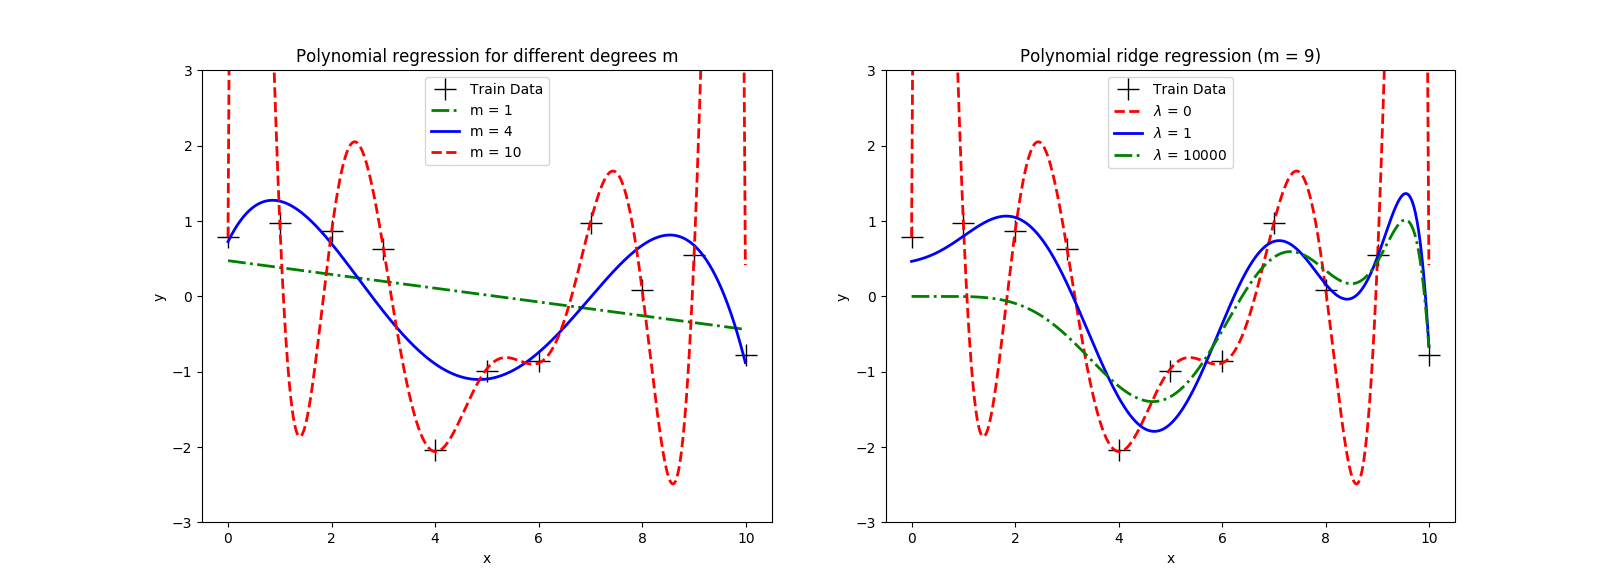
\includegraphics{Figure_1.png}
\caption{Figure\_1}
\end{figure}

    \begin{Verbatim}[commandchars=\\\{\}]
{\color{incolor}In [{\color{incolor}213}]:} \PY{k}{def} \PY{n+nf}{plot\PYZus{}style}\PY{p}{(}\PY{p}{)}\PY{p}{:}
              \PY{n}{plt}\PY{o}{.}\PY{n}{tight\PYZus{}layout}\PY{p}{(}\PY{p}{)}
              \PY{n}{pl}\PY{o}{.}\PY{n}{ylim}\PY{p}{(}\PY{o}{\PYZhy{}}\PY{l+m+mi}{3}\PY{p}{,} \PY{l+m+mi}{3}\PY{p}{)}
              \PY{n}{pl}\PY{o}{.}\PY{n}{xlabel}\PY{p}{(}\PY{l+s+s1}{\PYZsq{}}\PY{l+s+s1}{x}\PY{l+s+s1}{\PYZsq{}}\PY{p}{)}
              \PY{n}{pl}\PY{o}{.}\PY{n}{ylabel}\PY{p}{(}\PY{l+s+s1}{\PYZsq{}}\PY{l+s+s1}{y}\PY{l+s+s1}{\PYZsq{}}\PY{p}{)}
              \PY{n}{pl}\PY{o}{.}\PY{n}{legend}\PY{p}{(}\PY{n}{loc} \PY{o}{=} \PY{l+s+s1}{\PYZsq{}}\PY{l+s+s1}{upper center}\PY{l+s+s1}{\PYZsq{}}\PY{p}{)}
              
          \PY{k}{def} \PY{n+nf}{datapoint}\PY{p}{(}\PY{p}{)}\PY{p}{:}
              \PY{n}{X} \PY{o}{=} \PY{n}{sp}\PY{o}{.}\PY{n}{arange}\PY{p}{(}\PY{l+m+mi}{10}\PY{p}{)}
              \PY{n}{Y\PYZus{}train} \PY{o}{=} \PY{n}{sp}\PY{o}{.}\PY{n}{sin}\PY{p}{(}\PY{n}{X}\PY{p}{)} \PY{o}{+} \PY{n}{sp}\PY{o}{.}\PY{n}{random}\PY{o}{.}\PY{n}{normal}\PY{p}{(}\PY{l+m+mi}{0}\PY{p}{,}\PY{l+m+mf}{0.5}\PY{p}{,}\PY{n}{X}\PY{o}{.}\PY{n}{shape}\PY{p}{)}
              \PY{k}{return} \PY{n}{X}\PY{p}{,}\PY{n}{Y\PYZus{}train}\PY{p}{;}
          
          \PY{k}{def} \PY{n+nf}{getdata}\PY{p}{(}\PY{n}{X}\PY{p}{,}\PY{n}{Y\PYZus{}train}\PY{p}{,}\PY{n}{m}\PY{p}{,}\PY{n}{lam}\PY{p}{)}\PY{p}{:}
               \PY{c+c1}{\PYZsh{}the data matrix contains powers of the x coordinates of the data generated}
                  \PY{n}{X\PYZus{}train} \PY{o}{=} \PY{n}{sp}\PY{o}{.}\PY{n}{ones}\PY{p}{(}\PY{p}{(}\PY{l+m+mi}{1}\PY{p}{,}\PY{l+m+mi}{10}\PY{p}{)}\PY{p}{)}
                  \PY{k}{for} \PY{n}{k} \PY{o+ow}{in} \PY{n+nb}{range}\PY{p}{(}\PY{l+m+mi}{1}\PY{p}{,}\PY{n}{m}\PY{o}{+}\PY{l+m+mi}{1}\PY{p}{)}\PY{p}{:}
                      \PY{n}{X\PYZus{}train} \PY{o}{=} \PY{n}{sp}\PY{o}{.}\PY{n}{vstack}\PY{p}{(}\PY{p}{(}\PY{n}{X\PYZus{}train}\PY{p}{,}\PY{n}{X}\PY{o}{*}\PY{o}{*}\PY{n}{k}\PY{p}{)}\PY{p}{)}  
                  \PY{n}{W} \PY{o}{=} \PY{n}{train\PYZus{}ols}\PY{p}{(}\PY{n}{X\PYZus{}train}\PY{p}{,} \PY{n}{Y\PYZus{}train}\PY{p}{,}\PY{n}{llambda}\PY{o}{=}\PY{n}{lam}\PY{p}{)}
          
                  \PY{c+c1}{\PYZsh{}testing}
                  \PY{n}{N}\PY{o}{=}\PY{l+m+mi}{100} \PY{c+c1}{\PYZsh{}number of lattice nodes}
                  \PY{n}{Xt} \PY{o}{=} \PY{n}{sp}\PY{o}{.}\PY{n}{linspace}\PY{p}{(}\PY{l+m+mi}{0}\PY{p}{,}\PY{l+m+mi}{9}\PY{p}{,}\PY{n}{N}\PY{p}{)}
                  \PY{n}{X\PYZus{}test} \PY{o}{=} \PY{n}{sp}\PY{o}{.}\PY{n}{ones}\PY{p}{(}\PY{p}{(}\PY{l+m+mi}{1}\PY{p}{,}\PY{n}{N}\PY{p}{)}\PY{p}{)}
                  \PY{k}{for} \PY{n}{k} \PY{o+ow}{in} \PY{n+nb}{range}\PY{p}{(}\PY{l+m+mi}{1}\PY{p}{,}\PY{n}{m}\PY{o}{+}\PY{l+m+mi}{1}\PY{p}{)}\PY{p}{:}
                      \PY{n}{X\PYZus{}test} \PY{o}{=} \PY{n}{sp}\PY{o}{.}\PY{n}{vstack}\PY{p}{(}\PY{p}{(}\PY{n}{X\PYZus{}test}\PY{p}{,}\PY{n}{Xt}\PY{o}{*}\PY{o}{*}\PY{n}{k}\PY{p}{)}\PY{p}{)}        
                  \PY{n}{Y\PYZus{}test} \PY{o}{=} \PY{n}{apply\PYZus{}ols}\PY{p}{(}\PY{n}{W}\PY{p}{,} \PY{n}{X\PYZus{}test}\PY{p}{)}
                  \PY{k}{return} \PY{n}{Xt}\PY{p}{,}\PY{n}{Y\PYZus{}test}\PY{p}{;}
          
          \PY{k}{def} \PY{n+nf}{test\PYZus{}polynomial\PYZus{}regression}\PY{p}{(}\PY{p}{)}\PY{p}{:}
              
              \PY{c+c1}{\PYZsh{}generate toy data}
              \PY{n}{X}\PY{p}{,}\PY{n}{Y\PYZus{}train} \PY{o}{=} \PY{n}{datapoint}\PY{p}{(}\PY{p}{)}\PY{p}{;}
              
              \PY{n}{pl}\PY{o}{.}\PY{n}{figure}\PY{p}{(}\PY{n}{figsize}\PY{o}{=}\PY{p}{(}\PY{l+m+mi}{12}\PY{p}{,}\PY{l+m+mi}{8}\PY{p}{)}\PY{p}{)}
              \PY{o}{/}\PY{o}{/} \PY{n}{M} \PY{n}{subplot}
              \PY{n}{pl}\PY{o}{.}\PY{n}{subplot}\PY{p}{(}\PY{l+m+mi}{2}\PY{p}{,}\PY{l+m+mi}{2}\PY{p}{,}\PY{l+m+mi}{1}\PY{p}{)}
              \PY{n}{pl}\PY{o}{.}\PY{n}{plot}\PY{p}{(}\PY{n}{X}\PY{p}{,}\PY{n}{Y\PYZus{}train}\PY{p}{,}\PY{l+s+s1}{\PYZsq{}}\PY{l+s+s1}{+}\PY{l+s+s1}{\PYZsq{}}\PY{p}{,} \PY{n}{label} \PY{o}{=} \PY{l+s+s1}{\PYZsq{}}\PY{l+s+s1}{Train Data}\PY{l+s+s1}{\PYZsq{}}\PY{p}{)}
              
              \PY{k}{for} \PY{n}{m} \PY{o+ow}{in} \PY{p}{[}\PY{l+m+mi}{1}\PY{p}{,}\PY{l+m+mi}{4}\PY{p}{,}\PY{l+m+mi}{9}\PY{p}{]} \PY{p}{:}\PY{c+c1}{\PYZsh{}order of the polynomial}
                  \PY{c+c1}{\PYZsh{}training}
                  \PY{c+c1}{\PYZsh{}the data matrix contains powers of the x coordinates of the data generated}
                  \PY{n}{Xt}\PY{p}{,}\PY{n}{Y\PYZus{}test} \PY{o}{=} \PY{n}{getdata}\PY{p}{(}\PY{n}{X}\PY{p}{,}\PY{n}{Y\PYZus{}train}\PY{p}{,} \PY{n}{m}\PY{p}{,}\PY{l+m+mi}{0}\PY{p}{)}
              
                  \PY{k}{if} \PY{n}{m} \PY{o}{==} \PY{l+m+mi}{1}\PY{p}{:}
                       \PY{n}{pl}\PY{o}{.}\PY{n}{plot}\PY{p}{(}\PY{n}{Xt}\PY{p}{,}\PY{n}{Y\PYZus{}test}\PY{p}{,} \PY{n}{dashes}\PY{o}{=}\PY{p}{[}\PY{l+m+mi}{2}\PY{p}{,} \PY{l+m+mi}{2}\PY{p}{,} \PY{l+m+mi}{10}\PY{p}{,} \PY{l+m+mi}{2}\PY{p}{]}\PY{p}{,} \PY{n}{label} \PY{o}{=} \PY{l+s+s1}{\PYZsq{}}\PY{l+s+s1}{m=1}\PY{l+s+s1}{\PYZsq{}}\PY{p}{)}
                  \PY{k}{elif} \PY{n}{m} \PY{o}{==} \PY{l+m+mi}{4}\PY{p}{:}
                       \PY{n}{pl}\PY{o}{.}\PY{n}{plot}\PY{p}{(}\PY{n}{Xt}\PY{p}{,}\PY{n}{Y\PYZus{}test}\PY{p}{,} \PY{l+s+s1}{\PYZsq{}}\PY{l+s+s1}{b}\PY{l+s+s1}{\PYZsq{}}\PY{p}{,} \PY{n}{label} \PY{o}{=} \PY{l+s+s1}{\PYZsq{}}\PY{l+s+s1}{m=4}\PY{l+s+s1}{\PYZsq{}}\PY{p}{)}
                  \PY{k}{elif} \PY{n}{m} \PY{o}{==} \PY{l+m+mi}{9}\PY{p}{:}
                       \PY{n}{pl}\PY{o}{.}\PY{n}{plot}\PY{p}{(}\PY{n}{Xt}\PY{p}{,}\PY{n}{Y\PYZus{}test}\PY{p}{,} \PY{n}{dashes}\PY{o}{=}\PY{p}{[}\PY{l+m+mi}{6}\PY{p}{,} \PY{l+m+mi}{2}\PY{p}{]}\PY{p}{,} \PY{n}{label} \PY{o}{=} \PY{l+s+s1}{\PYZsq{}}\PY{l+s+s1}{m=10}\PY{l+s+s1}{\PYZsq{}}\PY{p}{)}
              
              \PY{n}{plot\PYZus{}style}\PY{p}{(}\PY{p}{)}\PY{p}{;}
              
              \PY{c+c1}{\PYZsh{}Lambda subplot}
              \PY{n}{pl}\PY{o}{.}\PY{n}{subplot}\PY{p}{(}\PY{l+m+mi}{2}\PY{p}{,}\PY{l+m+mi}{2}\PY{p}{,}\PY{l+m+mi}{2}\PY{p}{)}
              \PY{n}{pl}\PY{o}{.}\PY{n}{plot}\PY{p}{(}\PY{n}{X}\PY{p}{,}\PY{n}{Y\PYZus{}train}\PY{p}{,}\PY{l+s+s1}{\PYZsq{}}\PY{l+s+s1}{+}\PY{l+s+s1}{\PYZsq{}}\PY{p}{,} \PY{n}{label} \PY{o}{=} \PY{l+s+s1}{\PYZsq{}}\PY{l+s+s1}{Train Data}\PY{l+s+s1}{\PYZsq{}}\PY{p}{)}
              
              \PY{k}{for} \PY{n}{lam} \PY{o+ow}{in} \PY{p}{[}\PY{l+m+mi}{0}\PY{p}{,}\PY{l+m+mi}{1}\PY{p}{,}\PY{l+m+mi}{10000}\PY{p}{]} \PY{p}{:}\PY{c+c1}{\PYZsh{}value of lambda}
                  \PY{c+c1}{\PYZsh{}training}
                  \PY{n}{m} \PY{o}{=} \PY{l+m+mi}{9}
                  \PY{n}{Xt}\PY{p}{,}\PY{n}{Y\PYZus{}test} \PY{o}{=} \PY{n}{getdata}\PY{p}{(}\PY{n}{X}\PY{p}{,}\PY{n}{Y\PYZus{}train}\PY{p}{,} \PY{n}{m}\PY{p}{,}\PY{n}{lam}\PY{p}{)}
                  \PY{k}{if} \PY{n}{lam} \PY{o}{==} \PY{l+m+mi}{0}\PY{p}{:}
                       \PY{n}{pl}\PY{o}{.}\PY{n}{plot}\PY{p}{(}\PY{n}{Xt}\PY{p}{,}\PY{n}{Y\PYZus{}test}\PY{p}{,} \PY{n}{dashes}\PY{o}{=}\PY{p}{[}\PY{l+m+mi}{2}\PY{p}{,} \PY{l+m+mi}{2}\PY{p}{,} \PY{l+m+mi}{10}\PY{p}{,} \PY{l+m+mi}{2}\PY{p}{]}\PY{p}{,} \PY{n}{label} \PY{o}{=} \PY{l+s+s1}{\PYZsq{}}\PY{l+s+s1}{lambda=0}\PY{l+s+s1}{\PYZsq{}}\PY{p}{)}
                  \PY{k}{elif} \PY{n}{lam} \PY{o}{==} \PY{l+m+mi}{1}\PY{p}{:}
                       \PY{n}{pl}\PY{o}{.}\PY{n}{plot}\PY{p}{(}\PY{n}{Xt}\PY{p}{,}\PY{n}{Y\PYZus{}test}\PY{p}{,} \PY{l+s+s1}{\PYZsq{}}\PY{l+s+s1}{b}\PY{l+s+s1}{\PYZsq{}}\PY{p}{,} \PY{n}{label} \PY{o}{=} \PY{l+s+s1}{\PYZsq{}}\PY{l+s+s1}{lambda=1}\PY{l+s+s1}{\PYZsq{}}\PY{p}{)}
                  \PY{k}{elif} \PY{n}{lam} \PY{o}{==} \PY{l+m+mi}{10000}\PY{p}{:}
                       \PY{n}{pl}\PY{o}{.}\PY{n}{plot}\PY{p}{(}\PY{n}{Xt}\PY{p}{,}\PY{n}{Y\PYZus{}test}\PY{p}{,} \PY{n}{dashes}\PY{o}{=}\PY{p}{[}\PY{l+m+mi}{6}\PY{p}{,} \PY{l+m+mi}{2}\PY{p}{]}\PY{p}{,} \PY{n}{label} \PY{o}{=} \PY{l+s+s1}{\PYZsq{}}\PY{l+s+s1}{lambda=10000}\PY{l+s+s1}{\PYZsq{}}\PY{p}{)}
                          
              \PY{n}{plot\PYZus{}style}\PY{p}{(}\PY{p}{)}\PY{p}{;}
\end{Verbatim}


    \begin{Verbatim}[commandchars=\\\{\}]
{\color{incolor}In [{\color{incolor}214}]:} \PY{n}{test\PYZus{}polynomial\PYZus{}regression}\PY{p}{(}\PY{p}{)}  
\end{Verbatim}


    \begin{center}
    \adjustimage{max size={0.9\linewidth}{0.9\paperheight}}{output_24_0.pdf}
    \end{center}
    { \hspace*{\fill} \\}
    
    \textbf{B) (9 points)} Run your code of task A) multiple times. - (4
points) What do you observe for the different values of the parameters
\(m\) and \(\lambda\)? Explain this behaviour. - (2 points) Decide for
each of the two figures which values of the parameters yield the best
fit. - (3 points) Do you expect those parameters to perform good on all
possible data sets? Explain your decision.

    Answer : 1. \(m\)=1, hardly fits any data point \(m\)=4, fit couple of
data points \(m\)=9, fit every data point nicelly. \(m\) basically
determines the degree of polynomial to fit all the training data point
but the higher degree of \(m\) may lead to overfitting of test data and
may increase the test error. Also less dgree of \(m\) could lead to the
problem of Underfitting. \(\lambda\) = 0, fits all the data nicely
\(\lambda\) = 1, fir couple of data \(\lambda\) = 100000, hardly fit any
data point Having low value of \(\lambda\) gives more flexibility but
again that can lead to the overfitting problem and higher value of
\(\lambda\) could lead to the problem of Underfitting.

\begin{enumerate}
\def\labelenumi{\arabic{enumi}.}
\setcounter{enumi}{1}
\item
  The best fit is \(m\)=4 and \(\lambda\)=1.
\item
  No, parameters ought to change to fit the data points accuratley by
  avoiding both overfitting and Underfitting. These parameters will
  depend upon the type of data we have, suppose the data point is linear
  in that case lower value of \(m\) and higher value \(\lambda\) would
  be appropriate.
\end{enumerate}


    % Add a bibliography block to the postdoc
    
    
    
    \end{document}
